\label{sec:evaluation}

We evaluate \doubletake{} on a quiescent Intel Core 2 dual-processor system with 16GB of RAM running Linux 2.6.18-194.17.1.el5, and version 2.5 of \texttt{glibc}. Each processor is a 4-core 64-bit Intel Xeon, operating at 2.33GHz with a 4MB shared L2 cache a 32KB per-core L1 cache. All benchmarks are built as 64-bit executables using LLVM 3.2 with the clang front-end and \texttt{-O2} optimizations.

Our evaluation measure the memory and runtime overhead of \doubletake{}, and the effectiveness of the heap buffer overflow, memory leak, and use-after-free detectors.

\subsection{Performance Overhead}
\label{sec:perf}

\begin{figure*}[!ht]
	\begin{center}
		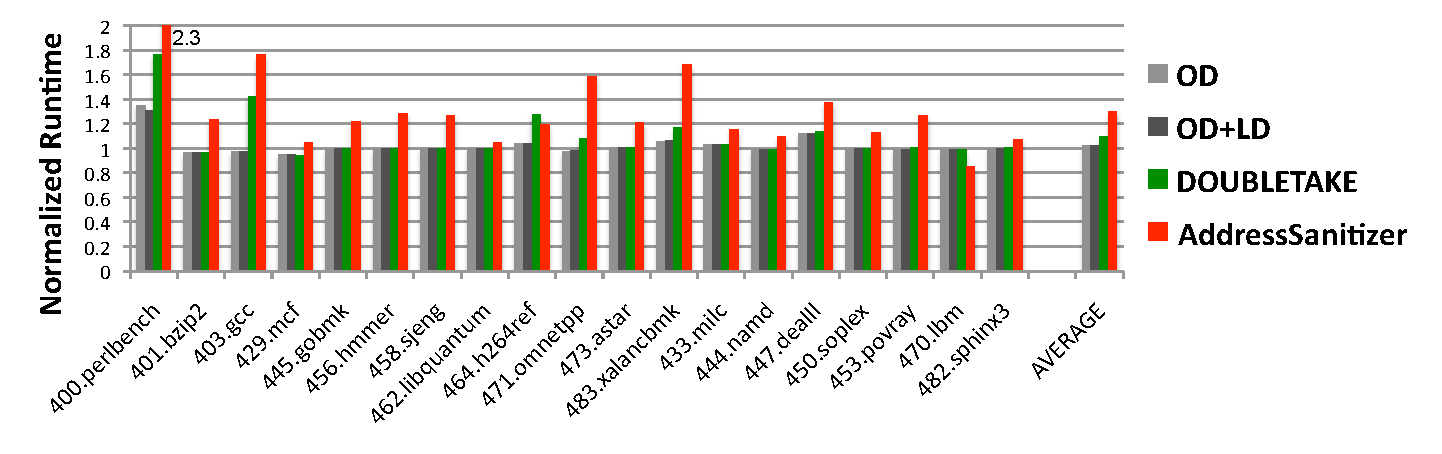
\includegraphics[width=6.5in]{doubletake/figure/perf}
	\end{center}
	\caption{This figure shows the runtime overhead of \doubletake{} (OD - Heap Overflows Detection, LD - Leak Detection, \doubletake{} - with three detections enabled) and AddressSanitizer, normalized to each benchmark's original execution time. 
%Overhead for Valgrind is reported in Table~\ref{table:valgrind} because the results do not fit on this graph.
\label{fig:perf}}
\end{figure*}

We evaluate performance on all C and C++ SPEC CPU2006 benchmarks, 19 in total. We compare \doubletake{} with AddressSanitizer and Valgrind. AddressSanitizer is the previous state-of-the-art for detecting buffer overflows and use-after-free errors~\cite{AddressSanitizer}, but cannot detect memory leaks. Valgrind's Memcheck tool is widely used tool to detect buffer overflows, memory leaks, and use-after-free errors~\cite{overflow:valgrind}. 

During performance evaluation, we disable \doubletake{}'s rollback to measure only the overhead of normal execution. \doubletake{}'s memory error detectors only run on the heap, so AddressSanitizer is run without checks on accesses to the stack and globals, and without checks on read accesses. For each benchmark, we report the average of three runs with the largest input size, except for Valgrind. We only run Valgrind once because of its slowness. 

Performance results of \doubletake{} and AddressSanitizer are shown in Figure~\ref{fig:perf}. Results for Valgrind do not fit on the graph, and are presented separately in Table~\ref{table:valgrind}. On average, \doubletake{} adds only $9\%$ overhead \emph{with all three error detectors enabled}. If \doubletake{} do not detect memory use-after-free errors, the performance overhead is under 3\% on average. AddressSanitizer slows execution by $30\%$ on average, and Valgrind has an average overhead of $19X$ on all evaluated benchmarks. Because Valgrind is running too slow, we haven't finished the evaluation on all benchmarks. Also, we kill a program if it is already running $20\times$ slower, including \texttt{400.perlbench} and \texttt{458.sjeng}. 

% difference across all different tools
For 17 out of 19 benchmarks, \doubletake{} outperforms AddressSanitizer, even with an additional memory leak detection. For 12 benchmarks, \doubletake{}'s runtime overhead is under 3\%. \doubletake{} substantially outperforms Valgrind for all benchmarks. For both \doubletake{} and AddressSanitizer,  \texttt{400.perlbench}, \texttt{403.gcc} and \texttt{447.deallIII} benchmark introduce much more performance overhead than other benchmarks. We also observe that they all introduce much more memory overhead (in terms of absolute value), according our experimental results in Table~\ref{tbl:memoryoverhead}. These significant memory overhead may reduce the ratio of cache efficiency, thus causing performance problem. 

% Difference across all different tools
From the figure, we also notice that detection of memory use-after-free adds about 6\% performance overhead averagely, although most of overhead are coming from \texttt{400.perlbench}, \texttt{403.gcc} and \texttt{464.h264ref} benchmark. As described in Section~\ref{sec:danglingpointer}, \doubletake{} has to fill every freed object up to 128 bytes with canaries and check those canaries when a freed object is released to the program heap. If an application has a big number of memory allocation and de-allocation, these operations consist of most of performance overhead. 

\begin{comment}
From the figure, we also observe that \doubletake{} introduces more than 7\% performance overhead for six benchmarks, including 400.perlbench, 403.gcc, 464.h264ref, 471.omnetpp, 483.xalancbmk, and 447.dealII. We further evaluate the overhead caused by different applications on these benchmarks. Results are showed in Figure ~\ref{fig:perfdetails}. From this figure, we observe that most overhead is coming from the component of detecting memory use-after-free errors. As described in Section~\ref{sec:danglingpointer}, \doubletake{} has to fill the first 128 bytes with canaries. If an application has a big number of memory allocation and de-allocation, filling canaries consists of the most significant overhead. When we remove the detection of memory use-after-free errors, performance overhead are dropping down from 9\% to less than 3\%, which are not shown here because of page limit. 

\begin{figure}
\begin{center}
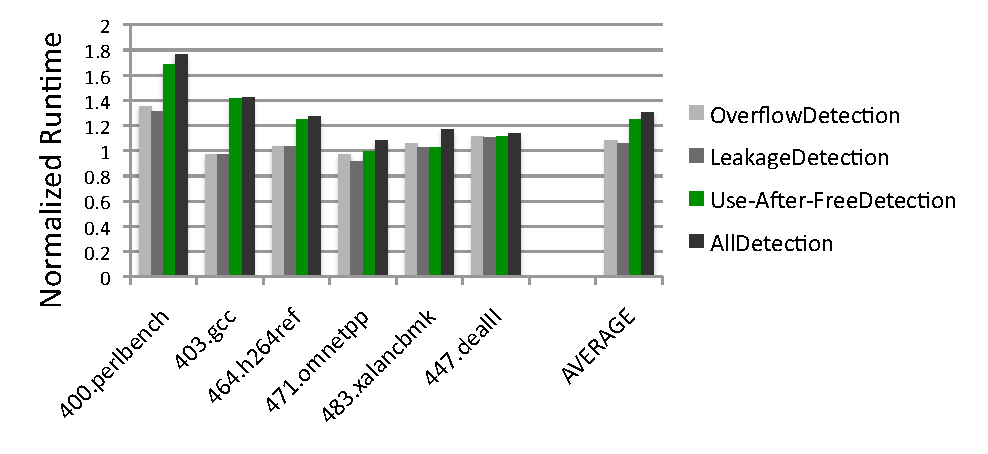
\includegraphics[width=3.4in]{doubletake/figure/perfdetails}
\end{center}
\caption{
\doubletake{} performance overhead for different applications.
\label{fig:perfdetails}}
\end{figure}

\end{comment}

\begin{table}[t]
	\centering
	\begin{tabular}{r|c p{0.1em} r|c}
		\textbf{Benchmark} & \textbf{Overhead} & & \textbf{Benchmark} & \textbf{Overhead} \\
		\cline{1-2} \cline{4-5}
		400.perlbench	& 20.5X	& & 458.sjeng	& 20.3X	\\
		401.bzip2		& 16.8X	& & 471.omnetpp	& 13.9X	\\
		403.gcc			& 18.7X	& & 473.astar	& 11.9X	\\
		429.mcf			& 4.5X 	& & 433.milc		& 11.0X	\\
		445.gobmk		& 28.9X	& & 444.namd		& 24.9X	\\
		456.hmmer		& 13.8X	& & 450.dealII	& 42.8X	\\
	\end{tabular}
	\caption{Valgrind's runtime overhead. \label{table:valgrind}}
\end{table}


\subsection{Memory Overhead}
\label{sec:memoverhead}

\begin{table}[t]
\centering
\begin{tabular}{l|c|c|c|}
\textbf{ \small Benchmark} & \textbf{\small Original} &  \textbf{\small AddressSanitizer} & \textbf{\small \doubletake{} } \\
\hline
400.perlbench & 656 &	1481 & 1977 \\
401.bzip2	& 870 &	1020 &	1003 \\
403.gcc	& 683 &	2293 &	1583 \\
429.mcf	& 1716 &	1951 &	1994 \\
445.gobmk &	28 &	137 &	58 \\
456.hmmer &	24 &	256 &	129 \\
458.sjeng & 179 & 220 &	203 \\
462.libquantum	& 66 &	144 &	131 \\
464.h264ref	& 65 &	179 &	247 \\
471.omnetpp	& 172 &	538 &	291 \\
473.astar	& 333 &	923 &	477 \\
483.xalancbmk &	428 & 1149 &	801 \\
433.milc	& 695 &	1008 &	917 \\
444.namd	& 46 &	79 &	92 \\
447.dealII	& 514 &	2496 &	1727 \\
450.soplex	& 441 &	1991 &	1654 \\
453.povray	& 3 &	133 &	50 \\
470.lbm	& 418 &	496 &	470 \\
482.sphinx3 &	45 &	181 & 98 \\
\hline
Total & 7386 & 16678 & 13906 \\
\hline
\end{tabular}
\caption{Memory Usage of \doubletake{} and AddressSanitizer(MB).\label{tbl:memoryoverhead}}
\end{table}


\begin{figure*}
\begin{center}
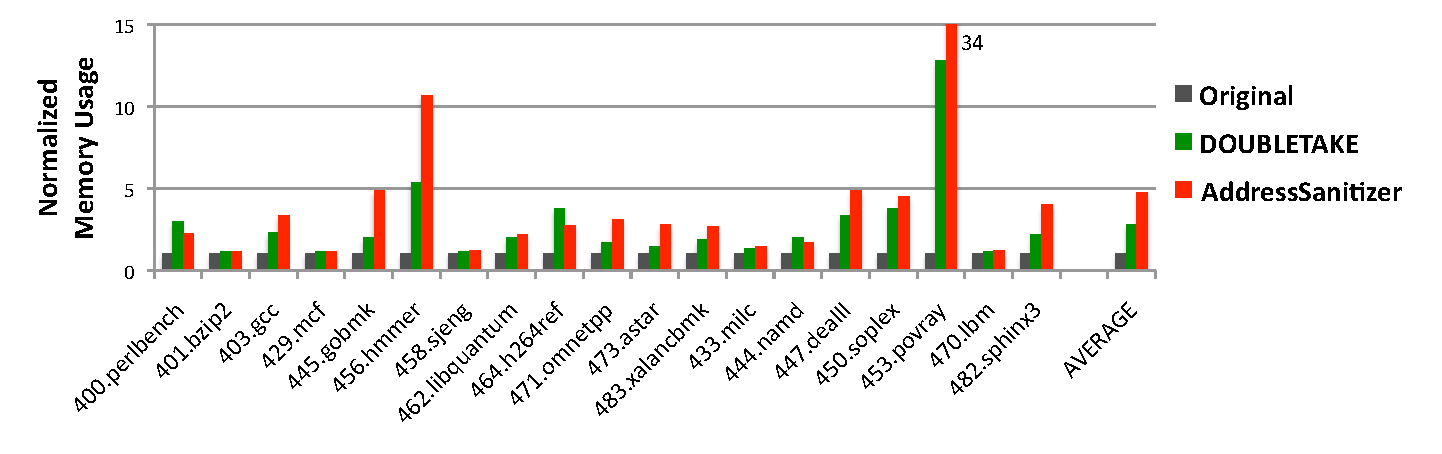
\includegraphics[width=6.5in]{doubletake/figure/memory}
\end{center}
\caption{
Memory overhead of \doubletake{} and AddressSanitizer.
\label{fig:memory}}
\end{figure*}

Memory overhead of \doubletake{} comes from the following aspects. Firstly, snapshot in the beginning of each epoch, by backing up the globals, the heap and the stack, contributes the most significant memory overhead of \doubletake{}. Snapshot can double the memory usage. However, the first snapshot happening in the beginning of a program normally doesn't take too much memory since there is no heap usage at all. Thus, this explains why \texttt{401.bzip2}, \texttt{429.mcf}, \texttt{458.sjeng},  \texttt{433.milc}, and \texttt{470.lbm} have less than $2\times$ memory overhead. Secondly, recording results of system calls introduce some memory overhead. Additionally, different applications may introduce different memory overhead. For the detection of heap buffer overflows and memory leakage, \doubletake{} adds canaries around each heap object and maintains a bit map to indicate canary locations. For the detection of memory usage-after-free errors, \doubletake{} delays memory re-usage by putting freed objects into a quarantine list, which also introduces constant additional memory overhead. 

We only evaluate the physical memory overhead here because \doubletake{} pre-allocates a huge block of heap, which is 4GB virtual memory and should not be counted as memory overhead. Also, we all only care about physical memory overhead when virtual memory overhead is practically infinite in 64bit machine. Proportional set size (PSS) in \texttt{/proc/self/smaps} reflects physical memory increase on the existing system by running an application. Thus, we periodically collect this data and use the sum of different memory mappings as total physical memory usage. We presents the normalized memory overhead of running different benchmarks in Figure~\ref{fig:memory}. We also list the actual memory usage of \doubletake{} and AddressSanitizer in Table~\ref{tbl:memoryoverhead}.

From Figure~\ref{fig:memory}, \doubletake{}'s memory overhead is 2.8$\times$, while AddressSanitizer's overhead is 4.8$\times$. For \texttt{453.povray} and \texttt{464.h264ref}, both AddressSanitizer and \doubletake{} has very high normalized memory overhead because the original memory usage of this benchmark is extremely low, only 3 and 24 megabytes. But for other benchmarks, both AddressSanitizer and \doubletake{} has memory overhead lesss than $5\times$. For all benchmarks except \texttt{400.perlbench} and \texttt{444.namd}, \doubletake{} has lower memory overhead. 
From Table~\ref{tbl:memoryoverhead}, AddressSanitizer totally spends about 20\% more memory than \doubletake{}. In total, \doubletake{} memory overhead is less than 2$\times$ of original memory usage. 

\subsection{Effectiveness}
\label{sec:effect}

\subsubsection{Micro Benchmarks}
All benchmarks evaluated in this subsection is taken from NIST SAMATE Reference Dataset Project ~\cite{microbenchmarks}.

{\bf Heap Overflows}: We evaluate \doubletake{} on 26 test cases listed in Table~\ref{table:SAMATESRDOverflow}. \doubletake{} can detect all buffer overflows when they corrupted canaries. \doubletake{} does not have any false alarms. Test cases 1955 and 2063 are not detected by \doubletake{} because they are not continuous buffer overflows, which cannot be detected by any canary-based approaches.

{\bf Memory Leakage}: We evaluate 13 test cases listed in Table~\ref{table:SAMATESRDLeak}. \doubletake{} reports memory leakage correctly for all test cases.  

{\bf Memory Usage-After-Free}: 
{Use After Free}
  
\begin{comment}

\begin{table}[!t]
\centering
\begin{tabular}{l|r}
\hline
{\bf \small Vunerbility Class} & {\bf \small SRD Test Case ID} \\
\hline
strcpy & 015 \\
strcpy & 1843 \\
strcpy & 1845 \\ % Array Index 
memory opration & 1952 \\ % Memory operation
Array Boundary & 1955 \\ % Array assignment
Array Boundary & 1958 \\ % Array assignment
Array Index & 1961 \\ % Array assignment
Array Index & 2062 \\ % Array assignment
Array Index & 2063 \\ % Array assignment
Array Index & 2064 \\ % Array assignment
Array Index & 2065 \\ % Array assignment
Array Index & 2145 \\ % Array assignment
strcpy & 2147 \\ % Array assignment

\hline \\ 
% Good Cases
strncpy & 1844 \\
strcpy & 1846 \\ % Array Index, limit string 
strcpy & 1848 \\
strcpy & 1936 \\
Memory & 1953 \\
Array Boundary & 1956 \\ % Array assignment
Array Boundary & 1959 \\ % Array assignment
Array Index & 1962 \\ % Array assignment
Array Index & 2066 \\ % Array assignment
Array Scope & 2067 \\ % Array assignment
Array Index & 2068 \\ % Array assignment
strcpy & 2134 \\ % Array assignment
strcpy & 2148 \\ % Array assignment
strcpy & 2149 \\ % Array assignment
 
\hline
\end{tabular}
\caption{SAMATE Test Cases. 
\label{table:SAMATESRD}}
\end{table}
\end{comment}


\begin{table}[!t]
\centering
\begin{tabular}{l|l}
\hline
{\bf \small Vulnerable Cases } & {\bf \small Good Cases} \\
\hline
015 1843 1845 1952 1955 & 1844 1846 1848 1936 1953\\
1958 1961 2062 2063 2065 & 1956 1959 1962 2066 2067 \\
2145 2147 & 2068 2134 2148 2149\\  
\hline
\end{tabular}
\caption{SAMATE Test Cases for Heap Overflows. 
\label{table:SAMATESRDOverflow}}
\end{table}

\begin{table}[!t]
\centering
\begin{tabular}{l|l}
\hline
{\bf \small Memory Leakage } & {\bf \small Good Cases} \\
\hline
1527 1583 1758 1925 1926 & 1458 1584 1587\\
1933 2056 99201 99202 99203 &   \\
\hline
\end{tabular}
\caption{SAMATE Test Cases for Memory Leakage. 
\label{table:SAMATESRDLeak}}
\end{table}

\begin{table}[!t]
\centering
\begin{tabular}{l|l}
\hline
{\bf \small Memory Leakage } & {\bf \small Good Cases} \\
\hline
1527 1583 1758 1925 1926 & 1458 1584 1587\\
1933 2056 99201 99202 99203 &   \\
\hline
\end{tabular}
\caption{SAMATE Test Cases for Memory Leakage. 
\label{table:SAMATESRDLeak}}
\end{table}

\subsubsection{Real Applications}

\begin{table}[!t]
\centering
\begin{tabular}{l|l|l}
\hline
{\bf \small Buffer Overflows} & {\bf \small Memory Leakage} & {\bf \small Use-after-free}\\
\hline
bc libhx & & \\
\hline
\end{tabular}
\caption{Evaluated Real Applications. 
\label{table:realapps}}
\end{table}

For buffer overflows, we have evaluate the effectiveness on  . Most of them have been included in
bugbench~\cite{}. 

For memory leakage problem, since we already found a lots of memory leakage in \texttt{perlbench}
and \texttt{gcc} benchmarks of SPEC2006, we evaluate real \texttt{perl} and \texttt{gcc} applications, {\bf PERL-... } and {\bf GCC-***} using the same input used in SPEC2006. 
Those memory leakage are still in these newest applications. 

For memory usage-after-free problems, 
In this section, we eveluate that 
LBC evaluate its effectiveness on bugbench.
bc, man and polymorph have overflow bugs.
gzip, ncompress exploit overflows using strcpy. 

%% RIPE: benchmark
%% Nullhttpd: two bound violations. We can't evaulate this problem because it is multithreaded program. 
%SAMATE:  

%Also, some from the Cruiser,
wu-ftpd, sudo, cvs, libhx, lynx
bc: two heap overflow
To check the effectiveness on the real applications, \doubletake{} evaluated all test cases listed in Table~\ref{}. They all coming from previous works. 


urrently, we have evaluated libhx successfully.

